\section{Analisi dei requisiti}
La presente sezione ha lo scopo di analizzare i servizi che il sito web finale deve offrire agli utenti e quali caratteristiche funzionali e qualitative devono essere garantite.

\subsection{Interazione degli utenti}
%cosa gli utenti possono fare? Quali attività/servizi offriamo?
Gli attori principali che interagiscono con il sito sono tre: l'utente comune, l'utente autenticato e il bibliotecario. Un utente è autenticato nel momento in cui possiede un account per il sito e ha effettuato la login, mentre il bibliotecario è un utente che ha effettuato l'accesso come amministratore. Di seguito sono descritti ad alto livello i casi d'uso principali che si sono previsti per ciascun attore.


\begin{figure}[H]
	\centering
	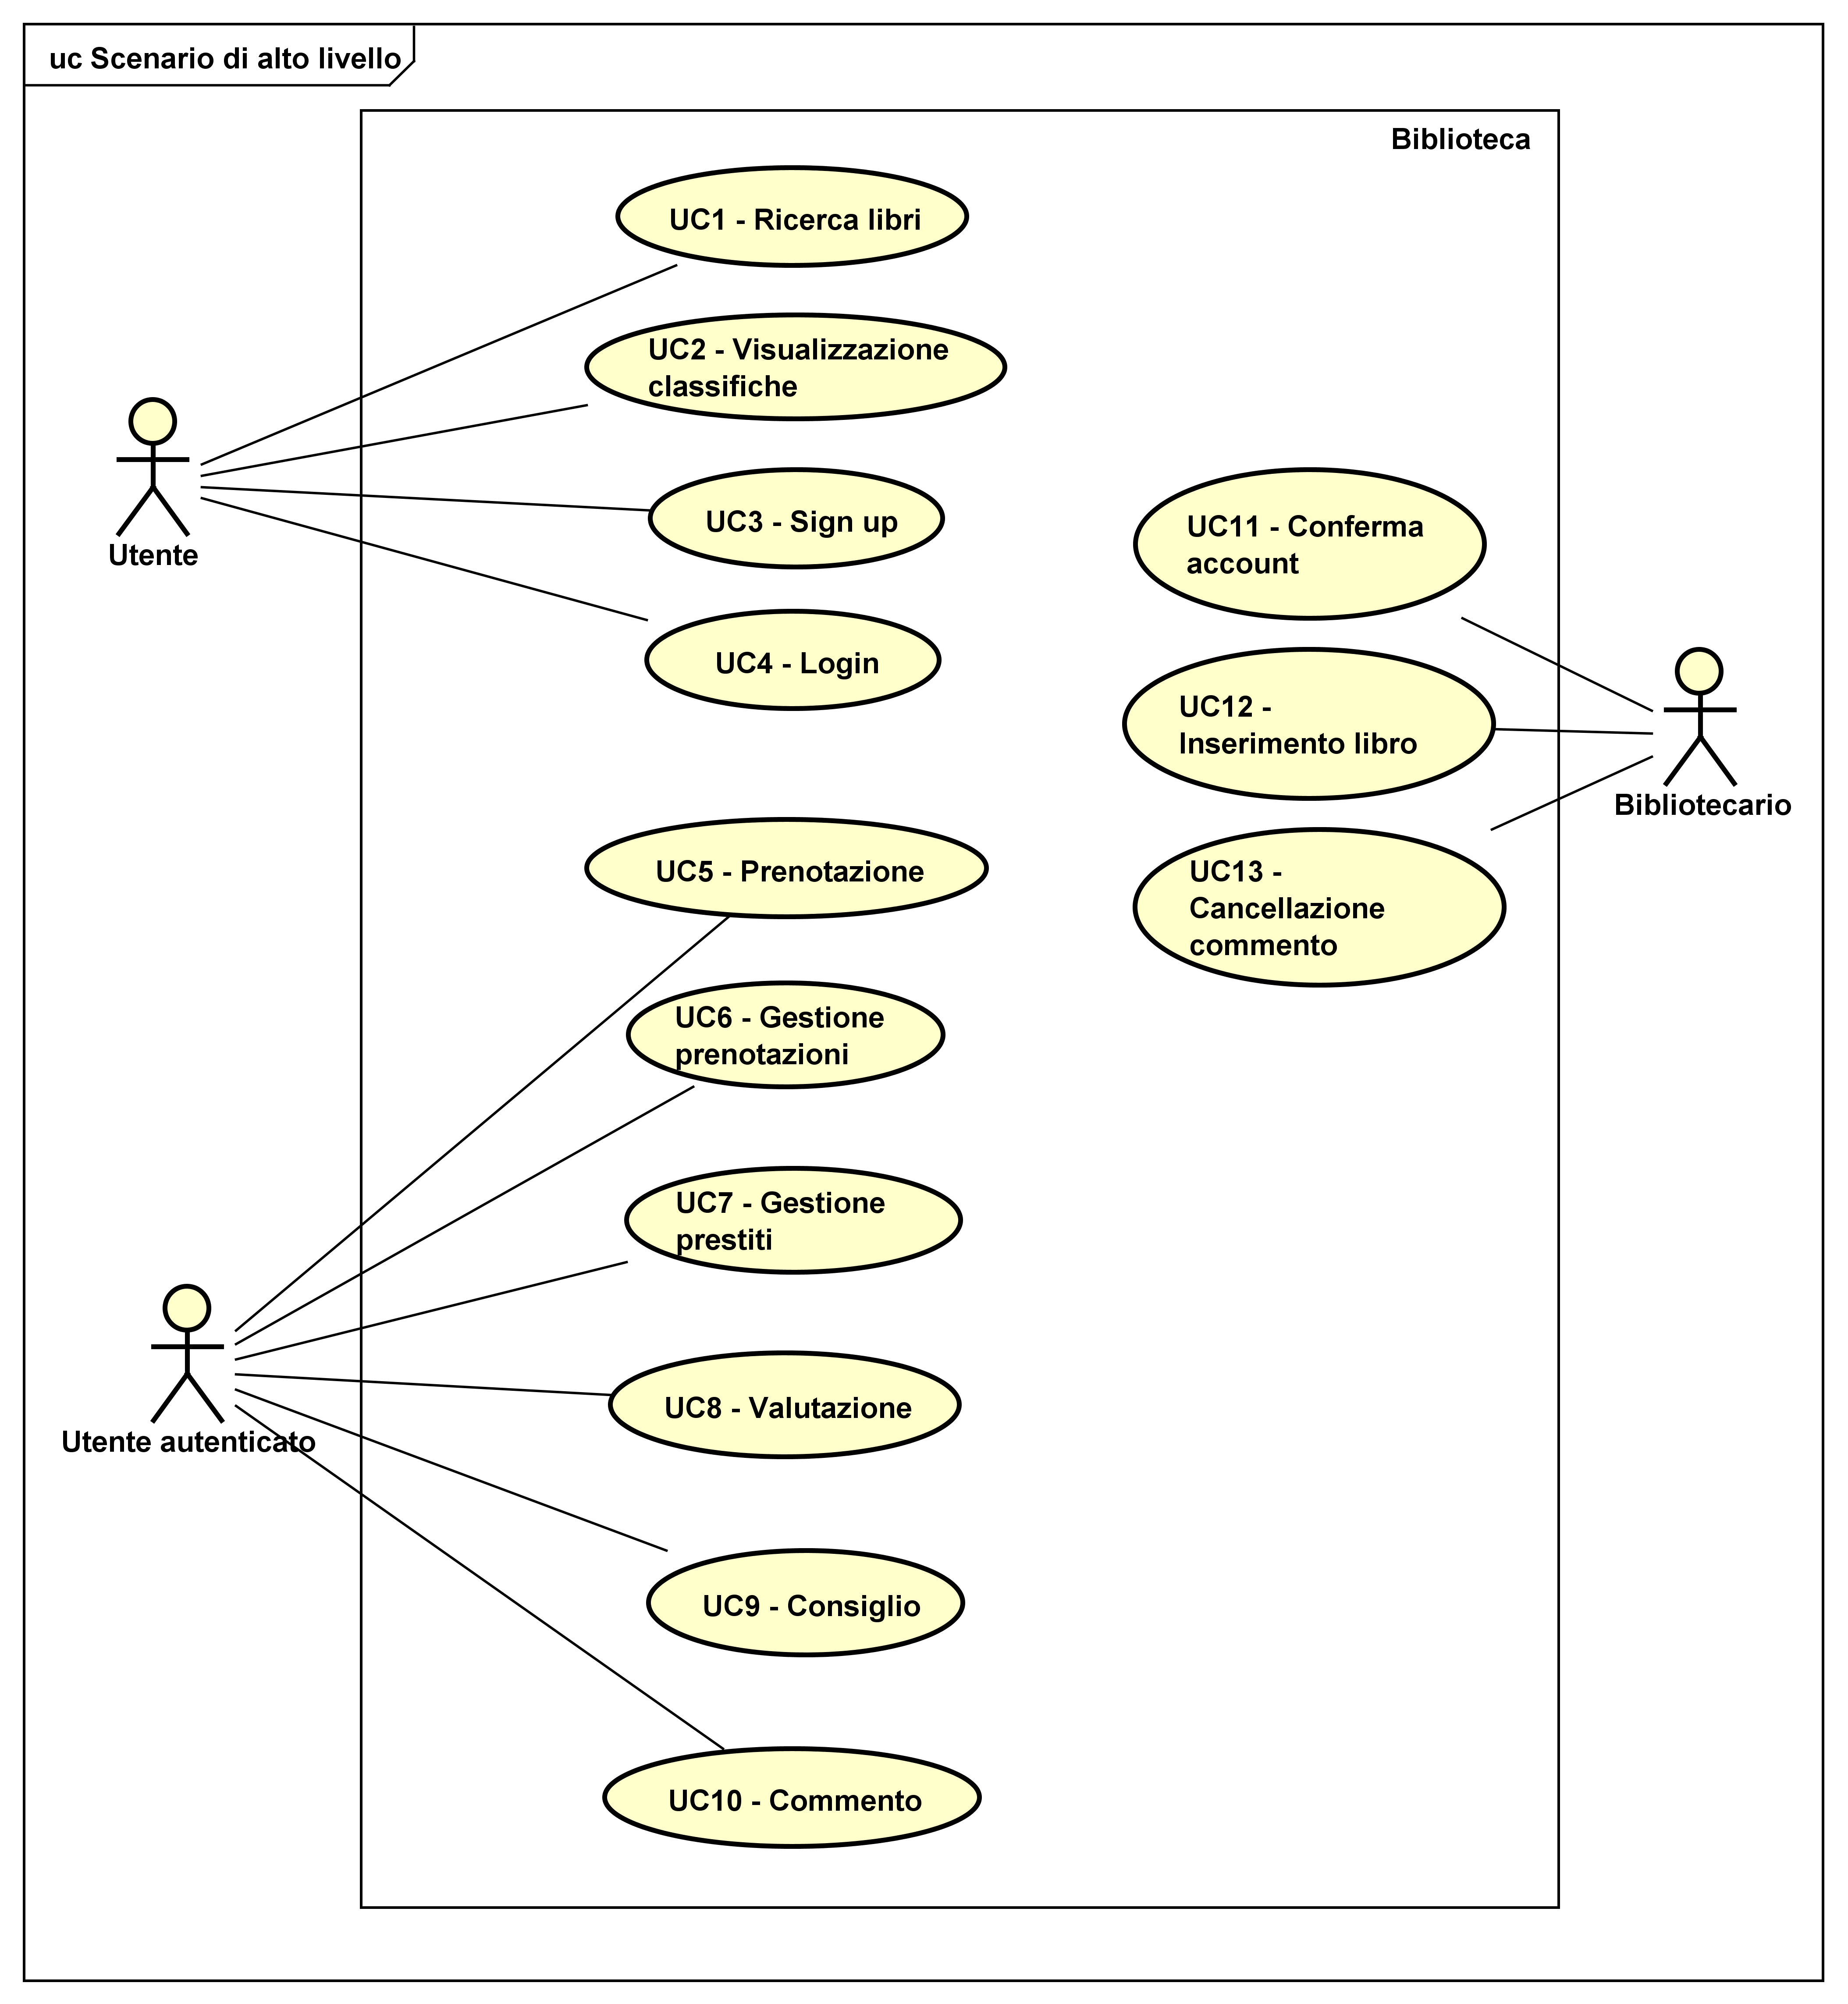
\includegraphics[width= 14cm]{immagini/user_case.png}
	\caption{Scenario di alto livello che mostra i principali casi d'uso.}
\end{figure}

\subsubsection{UC1 - Ricerca libri}
\begin{itemize}
	\item \textbf{Attore}: Utente;
	\item \textbf{Scopo e descrizione}: l'utente deve poter effettuare ricerche all'interno del sito. Deve essere garantita la ricerca per keyword, mentre opzionalmente si deve dare la possibilità di effettuare ricerche avanzate (in cui si possono cercare libri  o autori secondo attributi specifici). I risultati della ricerca devono essere mostrati in miniature che l'utente può espandere per avere maggiori informazioni se interessato;
	\item \textbf{Precondizione}: l'utente si trova nella pagina di ricerca;
	\item \textbf{Flusso principale degli eventi}:
	\begin{enumerate}
		\item l'utente inserisce una query di ricerca;
		\item l'utente avvia la ricerca premendo un opportuno bottone;
		\item vengono mostrati i risultati della ricerca;
		\item l'utente può riordinare i risultati della ricerca secondo un parametro (es. ordine alfabetico del titolo o data di pubblicazione).
	\end{enumerate} 
	\item \textbf{Postcondizione}: viene mostrato l'elenco di libri che soddisfa; la query;
	\item \textbf{Scenari alternativi}: nel caso la ricerca non portasse ad alcun risultato deve essere mostrato un messaggio informativo.
\end{itemize}

\subsubsection{UC2 - Visualizzazione classifiche}
\begin{itemize}
	\item \textbf{Attore}: Utente;
	\item \textbf{Scopo e descrizione}: l'utente deve poter visualizzare delle classifiche aggiornate sulle letture dei libri: i libri più letti, i libri più commentati, i libri più votati, le novità, i libri consigliati;
	\item \textbf{Precondizione}: esistono delle classifiche;
	\item \textbf{Flusso principale degli eventi}:
	\begin{enumerate}
		\item l'utente può visualizzare la classifica dei libri più letti, ossia i libri che sono stati prestati più volte;
		\item l'utente può visualizzare la classifica dei libri più commentati dagli utenti;
		\item l'utente può visualizzare la classifica dei libri più votati dagli utenti (in ordine di voto);
		\item l'utente può visualizzare la classifica delle novità;
		\item l'utente può visualizzare la classifica dei libri consigliati, ossia i libri che sono stati consigliati da più persone ad altri.
	\end{enumerate} 
	\item \textbf{Postcondizione}: viene mostrata la classifica richiesta.
\end{itemize}

\subsubsection{UC3 - Sign up}
\begin{itemize}
	\item \textbf{Attore}: Utente;
	\item \textbf{Scopo e descrizione}: l'utente deve potersi registrare nel sito inserendo una mail, uno username, una password e i propri dati. L'account viene confermato da un bibliotecario al momento della consegna del libro, con il rilascio di una tessera;
	\item \textbf{Precondizione}: l'utente ha un indirizzo mail;
	\item \textbf{Flusso principale degli eventi}:
	\begin{enumerate}
		\item l'utente inserisce il proprio nome;
		\item l'utente inserisce il proprio cognome;
		\item l'utente inserisce la propria età;
		\item l'utente inserisce il proprio indirizzo;
		\item l'utente inserisce il proprio indirizzo di posta elettronica;
		\item l'utente inserisce uno username;
		\item l'utente inserisce una password;
		\item l'utente conferma la password.
	\end{enumerate} 
	\item \textbf{Postcondizione}: viene creato un profilo non confermato.
\end{itemize}

\subsubsection{UC4 - Login}
\begin{itemize}
	\item \textbf{Attore}: Utente;
	\item \textbf{Scopo e descrizione}: l'utente deve potersi autenticare nel sito per accedere alle sue funzionalità principali: la prenotazione di libri, la gestione dei prestiti e i commenti;
	\item \textbf{Precondizione}: l'utente ha un account;
	\item \textbf{Flusso principale degli eventi}:
	\begin{enumerate}
		\item l'utente inserisce il proprio username;
		\item l'utente inserisce la propria password.
	\end{enumerate} 
	\item \textbf{Postcondizione}: l'utente è autenticato;
	\item \textbf{Scenari alternativi}: se le credenziali di accesso non sono corrette l'utente rimane non autenticato e gli viene chiesto di reinserire i dati.
\end{itemize}

\subsubsection{UC5 - Prenotazione}
\begin{itemize}
	\item \textbf{Attore}: Utente autenticato;
	\item \textbf{Scopo e descrizione}: l'utente autenticato deve poter prenotare un libro disponibile. Per la prenotazione deve essere indicata una data d'inizio, con limite massimo di un mese oltre la data corrente. Per un dato periodo può essere prenotato al massimo un libro;
	\item \textbf{Precondizione}: l'utente è autenticato
	\item \textbf{Flusso principale degli eventi}:
	\begin{enumerate}
		\item l'utente autenticato seleziona un libro;
		\item l'utente autenticato inserisce una data d'inizio per la prenotazione;
		\item l'utente autenticato inserisce una data di fine per la prenotazione;
		\item l'utente conferma la prenotazione.
	\end{enumerate} 
	\item \textbf{Postcondizione}: viene registrata una prenotazione;
	\item \textbf{Scenari alternativi}: se il libro non è più disponibile al momento della conferma, la prenotazione non viene effettuata.
\end{itemize}

\subsubsection{UC6 - Gestione prenotazioni}
\begin{itemize}
	\item \textbf{Attore}: Utente autenticato;
	\item \textbf{Scopo e descrizione}: l'utente autenticato deve poter cancellare una prenotazione esistente o modificarne le date prima di ritirare il libro;
	\item \textbf{Precondizione}: l'utente è autenticato ed ha effettuato una prenotazione;
	\item \textbf{Flusso principale degli eventi}:
	\begin{enumerate}
		\item l'utente può spostare la data d'inizio di una prenotazione purché non vada in collisione con altre prenotazioni esistenti;
		\item l'utente può spostare la data di fine di una prenotazione purché non vada in collisione con altre prenotazioni esistenti;
		\item l'utente può cancellare una prenotazione esistente.
	\end{enumerate} 
	\item \textbf{Postcondizione}: la prenotazione viene modificata o cancellata;
	\item \textbf{Scenari alternativi}: se la modifica delle date genera una collisione con altre prenotazioni esistenti non viene memorizzata.
\end{itemize}

\subsubsection{UC7 - Gestione prestiti}
\begin{itemize}
	\item \textbf{Attore}: Utente autenticato;
	\item \textbf{Scopo e descrizione}: l'utente autenticato deve poter visualizzare i dati relativi ai prestiti attivi in un dato momento; in particolare deve poter vedere le date di scadenza di ciascun libro in possesso. In aggiunta deve poter prorogare la consegna dei libri se questi non sono già prenotati da altri nel periodo indicato (entro un limite massimo); 
	\item \textbf{Precondizione}: l'utente è autenticato
	\item \textbf{Flusso principale degli eventi}:
	\begin{enumerate}
		\item l'utente autenticato può visualizzare l'elenco dei libri che ha attualmente in prestito;
		\item l'utente può visualizzare le date previste per la riconsegna di ciascun libro in prestito;
		\item l'utente autenticato può dilazionare un prestito se il libro non è prenotato.
	\end{enumerate} 
	\item \textbf{Postcondizione}: l'utente gestisce i propri prestiti.
\end{itemize}

\subsubsection{UC8 - Valutazione}
\begin{itemize}
	\item \textbf{Attore}: Utente autenticato;
	\item \textbf{Scopo e descrizione}: l'utente autenticato deve poter inserire un voto sui libri che ha preso in prestito;
	\item \textbf{Precondizione}: l'utente è autenticato e ha preso in prestito almeno un libro;
	\item \textbf{Flusso principale degli eventi}:
	\begin{enumerate}
		\item l'utente seleziona un libro fra quelli presi in prestito (dalla cronologia);
		\item l'utente inserisce una valutazione sul libro;
		\item l'utente conferma la valutazione.
	\end{enumerate} 
	\item \textbf{Postcondizione}: viene memorizzata la valutazione dell'utente sul libro.
\end{itemize}

\subsubsection{UC9 - Consiglio}
\begin{itemize}
	\item \textbf{Attore}: Utente autenticato;
	\item \textbf{Scopo e descrizione}: l'utente autenticato deve poter consigliare un libro preso in prestito ad un altro utente del sito.
	\item \textbf{Precondizione}: l'utente è autenticato, ha dei contatti ed ha preso in prestito un libro;
	\item \textbf{Flusso principale degli eventi}:
	\begin{enumerate}
		\item l'utente clicca sul pulsante "consiglia" di un libro;
		\item l'utente seleziona il contatto cui consigliare il libro;
	\end{enumerate} 
	\item \textbf{Postcondizione}: viene mandato un messaggio ad un utente del sito con il consiglio di lettura indicato.
\end{itemize}

\subsubsection{UC10 - Commento}
\begin{itemize}
	\item \textbf{Attore}: Utente autenticato;
	\item \textbf{Scopo e descrizione}: l'utente autenticato deve poter scrivere un commento sui libri che ha preso in prestito;
	\item \textbf{Precondizione}: l'utente è autenticato e ha preso in prestito un libro;
	\item \textbf{Flusso principale degli eventi}:
	\begin{enumerate}
		\item l'utente clicca sul pulsante "commenta" di un libro che ha preso in prestito;
		\item l'utente scrive il proprio commento;
		\item l'utente conferma l'invio del commento.
	\end{enumerate} 
	\item \textbf{Postcondizione}: viene memorizzato il commento dell'utente sul libro.
\end{itemize}

\subsubsection{UC11 - Conferma account}
\begin{itemize}
	\item \textbf{Attore}: Bibliotecario;
	\item \textbf{Scopo e descrizione}: un bibliotecario deve poter confermare un account al momento del rilascio di una tessera, inserendone il numero nell'apposito campo;
	\item \textbf{Precondizione}: l'utente ha un account non confermato;
	\item \textbf{Flusso principale degli eventi}:
	\begin{enumerate}
		\item il bibliotecario cerca il profilo non confermato;
		\item il bibliotecario inserisce il codice della tessera rilasciata;
		\item il bibliotecario conferma il profilo.
	\end{enumerate} 
	\item \textbf{Postcondizione}: viene confermato un account.
\end{itemize}

\subsubsection{UC12 - Inserimento libro}
\begin{itemize}
	\item \textbf{Attore}: Bibliotecario;
	\item \textbf{Scopo e descrizione}: un bibliotecario deve poter inserire un nuovo libro nella base di dati del sito;
	\item \textbf{Precondizione}: il bibliotecario è autenticato; 
	\item \textbf{Flusso principale degli eventi}:
	\begin{enumerate}
		\item il bibliotecario inserisce i dati del libro compilando un form;
		\item il bibliotecario conferma l'inserimento.
	\end{enumerate} 
	\item \textbf{Postcondizione}: viene memorizzato un nuovo libro.
\end{itemize}

\subsubsection{UC13 - Cancellazione commento}
\begin{itemize}
	\item \textbf{Attore}: Bibliotecario;
	\item \textbf{Scopo e descrizione}: il bibliotecario deve poter cancellare i commenti che reputa offensivi o inopportuni;
	\item \textbf{Precondizione}: sono memorizzati dei commenti;
	\item \textbf{Flusso principale degli eventi}:
	\begin{enumerate}
		\item il bibliotecario può cercare un commento;
		\item il bibliotecario può visualizzare l'elenco degli ultimi commenti inseriti;
		\item il bibliotecario può cancellare un commento.
	\end{enumerate} 
	\item \textbf{Postcondizione}: viene cancellato un commento.
\end{itemize}

\subsection{Aggiornamenti e amministrazione}
%definisci il progesso di aggiornamento del sito.. Come si aggiungono contenuti? Ogni quanto?
Gli utenti devono potersi registrare autonomamente nel sito, creando dei profili non confermati. Con tali account possono prenotare un libro e gestire la prenotazione. Una prenotazione diventa prestito al momento del ritiro del libro da parte dell'utente nella biblioteca. Contestualmente al primo ritiro di libri viene fornita una tessera (con identificativo univoco) all'utente. A questo punto un bibliotecario deve confermare il profilo dell'utente, inserendo il suo identificativo nell'apposita pagina di "conferma utenti" prevista nell'area amministrativa del sito.\\
Nella parte amministrativa deve essere infine fornita una pagina per inserire i libri, in modo da tenere aggiornato il sito sui contenuti della biblioteca. All'arrivo di nuovi libri il bibliotecario deve quindi poterne inserire i dati.


\subsection{Organizzazione e mappa del sito}
%che struttura ha il sito?
Il sito sarà composto dalle seguenti pagine:
\begin{itemize}
	\item \textbf{index.cgi}: homepage del sito..
	\item \textbf{contatti.html}: ..
	\item \textbf{catalogo.cgi}: ..
	\item \textbf{dettaglio\_libro.cgi}: ..
	\item \textbf{servizi.html}: ..
	\item \textbf{login.html}: ..
	\item \textbf{prenotazione.cgi}: ..
	\item \textbf{gestione\_prestito.cgi}: ..
	\item \textbf{profilo\_utente.cgi}: ..
	\item \textbf{conferma\_account.cgi}: nella parte di amministrazione..
	\item \textbf{inserimento\_libro.html}: ..
	\item \textbf{rimozione\_commento.cgi}: ..
\end{itemize}
I collegamenti fra le pagine, che determinano la navigazione nel sito sono descriti dal seguente diagramma:\\
\textbf{[inserire diagramma]}


\subsection{Performance}
%quali sono gli indicatori e cosa ci si aspetta


\subsection{Accessibilità}


\subsection{Sicurezza}